\subsection{Generic method}
\label{generic}

The generic method introduce a way more complex branching scheme but allow to keep subproblems with the knapsack structure. As the knapsack problem can be solve with dynamic programming, this will allow to have a faster resolution method for the subproblems.

\subsubsection{Branching rules}

When a node is solved to optimality and that two items $i$ and $j$ are found to create a branch, we have to create one child where $w_{ij} \leq 0$ (the down branch) and one child where $w_{ij} \geq 1$ (up branch). For the down branch, we will create a subproblem generating patterns with $x_i = 0$ and patterns with $x_i = 1, x_j=0$. Thus, the solution constructed will be constituted of patterns with items $i$ and $j$ separated. But we only need one pattern with $x_i = 1, x_j=0$ so we will also impose that 
\begin{equation}
	\label{generic-down}
	\left \{
	\begin{array}{l}
	\displaystyle \sum_{p \in \Pc' | x_i^p=1, x_j^p=0} \alpha^p = 1 \\
	\displaystyle \sum_{p \in \Pc' | x_i^p=0} \alpha^p = B-1 \\
	\end{array}
	\right.
\end{equation}
For the up branching rule, we will create one subproblem generating patterns with $x_i = x_j = 0$ and patterns with $x_i = x_j = 1$. Thus, the solution will be composed of patterns with $i$ and $j$ together (and patterns without $i$ and $j$). But we only need one pattern with $x_i = x_j = 1$ so we will also impose that
\begin{equation}	
	\label{generic-up}
	\left \{
	\begin{array}{l}
	\displaystyle \sum_{p \in \Pc' | x_i^p= x_j^p=1} \alpha^p = 1 \\
	\displaystyle \sum_{p \in \Pc' | x_i^p= x_j^p=0} \alpha^p = B-1 \\
	\end{array}
	\right.
\end{equation}
For up and down branching rules, we can notice that the variables $x_i$ and $x_j$ are fixed so the subproblem keep its knapsack structure if a preprocess is made. After fixing the branching variable, a knapsack problem will remained to be solved.

The difficulty lies in the method to process several branches in a row in the tree. We have to introduce the notion of \textbf{branching set} which are composed of some \textbf{branching rules} (corresponding to the filter below the sum in \eqref{generic-down} and \eqref{generic-up}) and one \textbf{coefficient} (corresponding to the scalar 1 or $B-1$ in \eqref{generic-down} and \eqref{generic-up}). Each branching rule has several variables set to zero and several variables set to one. For example, 
\begin{equation*}
	\sum_{p \in \Pc' | \{x_1 = 0, x_2 = 1\} \cup \{x_3 = 0, x_4 = 1\}} \alpha^p = 1
\end{equation*}
is a branching set with branching rules $\{x_1 = 0, x_2 = 1\}$ and $\{x_3 = 0, x_4 = 1\}$ and with coefficient $1$ and 
\begin{equation*}
	\sum_{p \in \Pc' | \{x_1 = x_2 = 0\}} \alpha^p = B-1
\end{equation*}
is a branching set with branching rule $\{x_1 = x_2 = 0\}$ and with coefficient $B-1$.

When a new node is created, we will loop over all the branching sets of the parent node and create new sets for the child node by adding the new branching rules. Four cases can happen : 

\begin{itemize}
	\item \textbf{The coefficient of the parent node set is L > 1} : \\
	In this case, the branching set have a unique rule by construction of the child nodes.
	\begin{itemize}
		\item \textbf{We have to add a down branching rule with items $i$ and $j$} : In this case, we will create two branching set for the child node. One with the same items set to one and zero as the parent node but we add the item $i$ to the variable set to 0. This branching set have a coefficient $\L-\1$. The second branching set will have the same items set to one and zero as the parent node but we add the item $i$ to the variable set to 1 and the item $j$ to the variable set to 0. This second branching set have a coefficient equal to $\1$.
	\end{itemize}
	\begin{itemize}
		\item \textbf{We have to add an up branching rule with items $i$ and $j$} : In this case, we will create two branching set for the child node. One with the same items set to one and zero as the parent node but we add the item $i$ and $j$ to the variable set to 0. This branching set have a coefficient $\L-\1$. The second branching set will have the same items set to one and zero as the parent node but we add the item $i$ and $j$ to the variable set to 1. This second branching set have a coefficient equal to $\1$.
	\end{itemize}
	\item \textbf{The coefficient of the parent node set is 1} : \\
	In this case, the branching set can have a multiple rule by construction of the child nodes so only one pattern satisfying one of the rule will be selected in the solution.
	\begin{itemize}
		\item \textbf{We have to add a down branching rule with items $i$ and $j$} : Only one set is created in the child node. For each branching rule in the parent node branching set, we add two new rule to the child branching set containing the rule of the parent branching set and either $x_i = 0$ or $x_i=1, x_j=0$. This new branching set has a coefficient equal to $1$.
	\end{itemize}
	\begin{itemize}
		\item \textbf{We have to add an up branching rule with items $i$ and $j$} : Only one set is created in the child node. For each branching rule in the parent node branching set, we add two new rule to the child branching set containing the rule of the parent branching set and either $x_i = x_j = 0$ or $x_i=x_j=1$. This new branching set has a coefficient equal to $1$.
	\end{itemize}
\end{itemize}

The way new constraints are added to the child nodes is a bit complicated as we have to handle multiple subproblems and we have to ensure that the coefficient of each branching set add to $B$ in order to satisfy the constraint $\sum_{p \in \Pc'} \alpha^p = B$ of \eqref{RMBPP} for each node. Of course, some of the rules created may be infeasible if one item is both in the set of variables set to 0 and 1. In this case, the rules is not included in the branching set. If the parent branching set is split into one feasible and one infeasible branching set, then we only keep the feasible branching set and the coefficient of the new set is equal to the coefficient of the parent branching set.
\begin{figure}[!ht]
	\centering
	\begin{minipage}{0.47\linewidth}
		\centering
		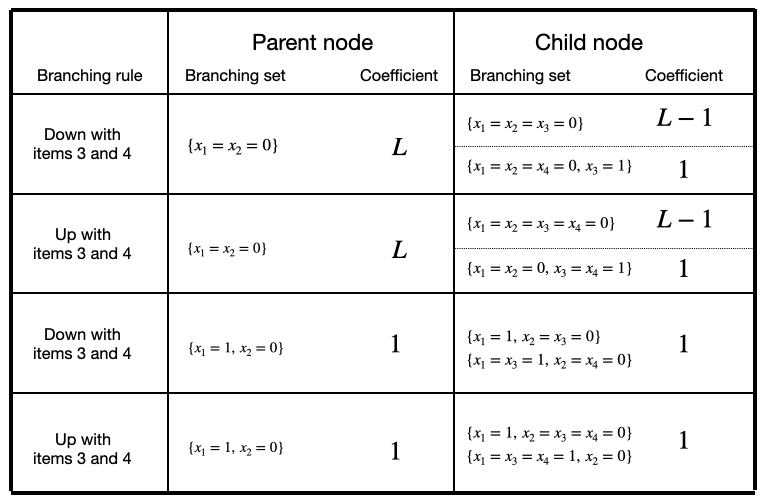
\includegraphics[width=0.7\linewidth]{img/generic-branching.png}
	\end{minipage}
	\begin{minipage}{0.47\linewidth}
		\centering
		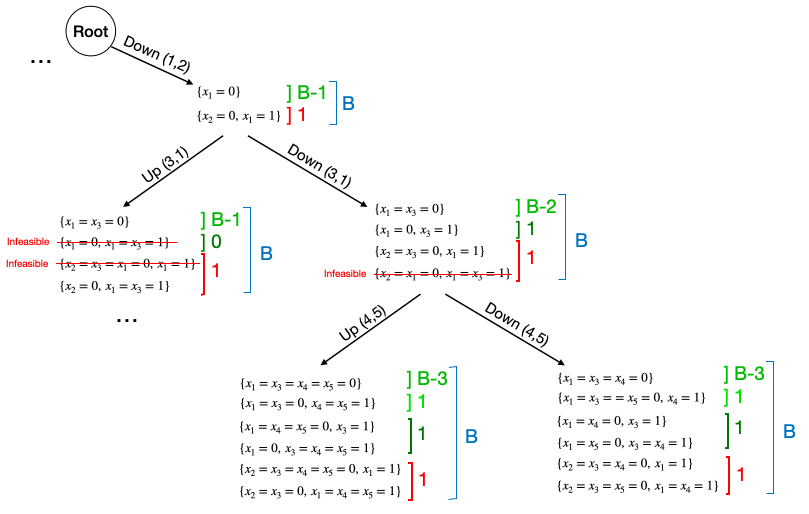
\includegraphics[width=\linewidth]{img/generic-example.png}
	\end{minipage}
	\caption{Left : The four cases presented above. Right : An example of how branching constraints are handled.}
\end{figure}

\subsubsection{Subproblem resolution}

In each node, there will be as many subproblems to solve as the total number of branching rules. As for the Ryan \& Foster branching method, it is possible to use a solver like Gurobi to solve the subproblems. It will preprocess the problem by setting the variables to 0 or 1 according to the branching schemes before the solving process. But as the knapsack structure is preserved for each subproblem, it is possible to use dynamic programming instead of a classical solver. 

The first step to do before the dynamic programming process is to preprocess the data and treat the variables already fixed by the branching rules. For each variable set to 0, we simply remove this variable from the problem. For each variable set to 1, we remove the variable from the problem, we also decrease the knapsack capacity by the size of the item and add its cost to a preprocess cost. At the end of the preprocess, if the capacity of the knapsack is still positive, then the dynamic programming process can start. If the capacity is negative, then the knapsack problem is infeasible and the resolution is stopped here. At the end of the dynamic programming process, the total cost is the cost outputted plus the preprocess cost and the items in the pattern are the items used in the knapsack solution plus the items set to 1 during the preprocess step.

To solve dynamically the knapsack problem considering a capacity $C^{knap}$, and items with sizes $s_i^{knap}$ and costs $p_i^{knap}$ for $i=1,\dots, I^{knap}$, we have to introduce $t_{i,c}^{knap}$, the maximal cost of a knapsack problem with cost $c$ and with $i$ items among all the items. We can apply the following dynamic programming algorithm and backtracking to find the optimal cost of the knapsack and the items involved in this optimal cost : 
\begin{figure}[!ht]
	\centering
	\begin{minipage}[t]{0.48\linewidth}
		\begin{algorithm}[H]
			\DontPrintSemicolon 
			\For{$i = 1,\dots, I^{knap}$}{
				\For{$c = 1,\dots,C^{knap}$}{
					\uIf{$s_i^{knap} > c$}{
						$t_{i+1,c} \leftarrow t_{i,c}$\;
					}\Else{
						$t_{i+1,c} \leftarrow \max \{t_{i,c} \ ; \  p_i^{knap} + t_{i,c-s_i^{knap}}\}$\;
					}
				}
			}
			\caption{Knapsack problem}
		\end{algorithm}
	\end{minipage}
	\hfill
	\begin{minipage}[t]{0.49\linewidth}
		\begin{algorithm}[H]
			\DontPrintSemicolon 
			Pattern $ \leftarrow \emptyset$\;
			$c = C^{knap}$\;
			\For{$i = I^{knap},\dots,1$}{
				\If{$t_{i,c} \neq t_{i-1,c}$}{
					Pattern $\leftarrow$ Pattern $\cup \ i$\;
					$c \leftarrow c -  s_i^{knap}$\;
				}
			}
			\caption{Knapsack problem, backtracking}
		\end{algorithm}
	\end{minipage}
\end{figure}

\noindent The optimal cost is $t_{I^{knap}, C^{knap}}$ and the variable $Pattern$ contains the items involved in the optimal cost.

We can observe that the complexity of the dynamic program is $o(I^{knap}C^{knap})$. Although it can be way better than solving the subproblem using a solver, some problems can happen when the capacity of the knapsack is large. The dynamic program is not only size-dependant but also data-dependant in the way that two problems with the same number won't be solved in the same amount of time. A problem with few items but with a huge capacity can be slower to solve than a problem with more items. In practice, it could be interesting to measure the solving time per number of items while using the solver and the solving time per number of items and capacity using dynamic programming in order to chose which solving method to chose. Furthermore, as the dynamic programming method is implemented "by hand" in this project while the solver have already been developed and optimized, the solver can still be faster in practice than the dynamic program even if the theoretical complexity is worst.